%% LaTeX_Thesis_Template.tex
% An unofficial LaTeX template for Cranfield theses.
% 2017/08/14 Daniel Auger's unofficial Cranfield thesis .sty file
% 2023/05/31 Updated by Shaun Forth (SAF) for logo inclusion
% 2023/06/08 SAF removed capitalisation on title pages on advice of Amy 
% Greenaway and Alison Waters. Added Daniel Auger's headers with 
% chapter and section names.
% 2023/06/08 SAF simplified logo inclusion

%%
% This document is an example of the use of the unofficial "cranfieldthesis" 
% LaTeX style file.  I hope it's useful, and a good likeness of the Word template.

\documentclass[12pt,oneside]{book} % for one-sided printing
%\documentclass[12pt,twoside]{book} % for two-sided printing

% Use the custom "cranfieldthesis" LaTeX style file. 
\usepackage{cranfieldthesis}
\usepackage{lscape} % for landscape pages
\usepackage{amsmath}
\usepackage{enumitem}
\usepackage{changepage}
\usepackage{pdfpages}
\usepackage{blindtext}% Just used so we can generate some example text
\usepackage{algorithm}
\usepackage{algpseudocode}
\usepackage{amssymb}
\usepackage{mathtools}
\usepackage[export]{adjustbox}
\usepackage{lipsum}
\usepackage{booktabs}  % For better quality tables
\usepackage{siunitx}
\usepackage{float}
\usepackage{longtable} % Pour les tableaux sur plusieurs pages
\usepackage{tabularx}  % for the X column type
\usepackage{listings}
\usepackage{xcolor}
\usepackage{caption}
\usepackage{xfrac}
\usepackage{indentfirst}
\usepackage{subcaption}
\usepackage{graphicx}
\usepackage{geometry}
\usepackage{titlesec}
\geometry{a4paper, margin=1in}
\hypersetup{
    colorlinks,
    linkcolor={blue!50!blue},
    citecolor={blue!50!blue},
    urlcolor={blue!80!blue}
}

% By default, LaTeX uses a serif font - these are traditionally thought to be
% easier to read.   If you'd prefer sans-serif, please uncomment the 
% following line.
% \renewcommand{\familydefault}{\sfdefault}

% Example parameters for a typical taught MSc course
\title{Future Position Prediction for Pressure Refuelling Port
    of Commercial Aircraft}
\author{Alexis Balayre}
\date{May 2024}
\school{\SATM}
\course{Computational and Software Techniques in Engineering}
\degree{MSc}
\academicyear{2023--2024}
\setCUPartnerLogo{logo-airbus.png}
\supervisors{Dr Boyu Kuang and Dr Stuart Barnes}
\copyrightyear{2024}

% References
% Cranfield Numbered Style
\usepackage[numbers]{natbib} % for nice referencing
\makeatletter % Reference list option change to number and period
\renewcommand\@biblabel[1]{#1.} % from [1] to 1
\makeatother %
\setcitestyle{numbers} % use round citations

\begin{document}

%% Front matter
%
% This is where we do the title page, etc.
%

\frontmatter

% Standard-Form Title Pages
\maketitle

% Abstract and Keywords
\begin{abstract}
    Replace with your abstract text of not more than 300 words.
\end{abstract}

\begin{keywords}
    Replace with at least 6, semicolon seperated keywords (not contained within the thesis title) – this makes the thesis searchable.
\end{keywords}

% Acknowledgements
\chapter{Acknowledgements}
The author would like to thank \dots

% Use single spacing for Table of Contents, List of Figures, etc
{
    \clearpage

    % Table of Contents
    \singlespacing{
        \tableofcontents
    }
    \clearpage

    % List of Figures
    \listoffigures

    \clearpage
    % List of Tables
    \listoftables
}

% The list of abbreviations can't be automatically generated so you need to populate it yourself
\begin{listofabbreviations}
    \abbrev{SATM}{School of Aerospace, Technology and Manufacturing}
    \abbrev{SEEA}{School of Energy, Environment and Agrifoods}
    \abbrev{CDS}{Cranfield Defence and Security}
\end{listofabbreviations}

%% Main Matter
%
% This is where we include the main thesis content.
%
\mainmatter\pagestyle{fancy}
\fancyhead[L]{\nouppercase{\leftmark}}
\fancyhead[R]{\nouppercase{\rightmark}}

\chapter{Introduction}

Ground pressure refuelling is a standard method used to refuel commercial
aircraft safely and efficiently. This process involves using a hydrant system,
which consists of underground fuel pipelines connected to a network of fuel
hydrants located at aircraft parking positions~\cite{blakey2011aviation}. The
hydrant system is supplied with fuel from storage tanks, typically located near
the airport~\cite{kazda2015airport}.

When an aircraft is ready for refueling, a hydrant dispenser vehicle, also
known as a hydrant truck or cart, is connected to the hydrant pit using a
flexible hose~\cite{sati2019aircraft}. The hydrant dispenser vehicle is
equipped with a pressure control valve, a flow meter, and a filtration system
to ensure that the fuel meets the required quality
standards~\cite{iata2019guidance}.

The refueling process begins by connecting the hydrant dispenser vehicle to the
aircraft's fuel panel using another flexible hose~\cite{sati2019aircraft}. The
pressure control valve on the hydrant dispenser vehicle is then used to
regulate the fuel pressure and flow rate, ensuring that the fuel is delivered
to the aircraft at the appropriate pressure and volume~\cite{iata2019guidance}.

One of the main advantages of pressure ground refueling is its efficiency. This
method allows for high fuel flow rates, which can significantly reduce aircraft
turnaround times~\cite{blakey2011aviation}. Additionally, the use of
underground pipelines eliminates the need for fuel trucks, reducing traffic
congestion and the risk of accidents on the apron~\cite{kazda2015airport}.

Safety is another critical aspect of pressure ground refueling. The hydrant
system is designed with multiple safety features, such as emergency shutdown
valves and leak detection systems, to minimise the risk of fuel spills and
fires~\cite{iata2019guidance}. Moreover, the hydrant dispenser vehicles are
equipped with safety devices, such as dead man switches and bonding cables, to
prevent incidents during the refueling process~\cite{sati2019aircraft}.

\begin{figure}[H]
    \centering
    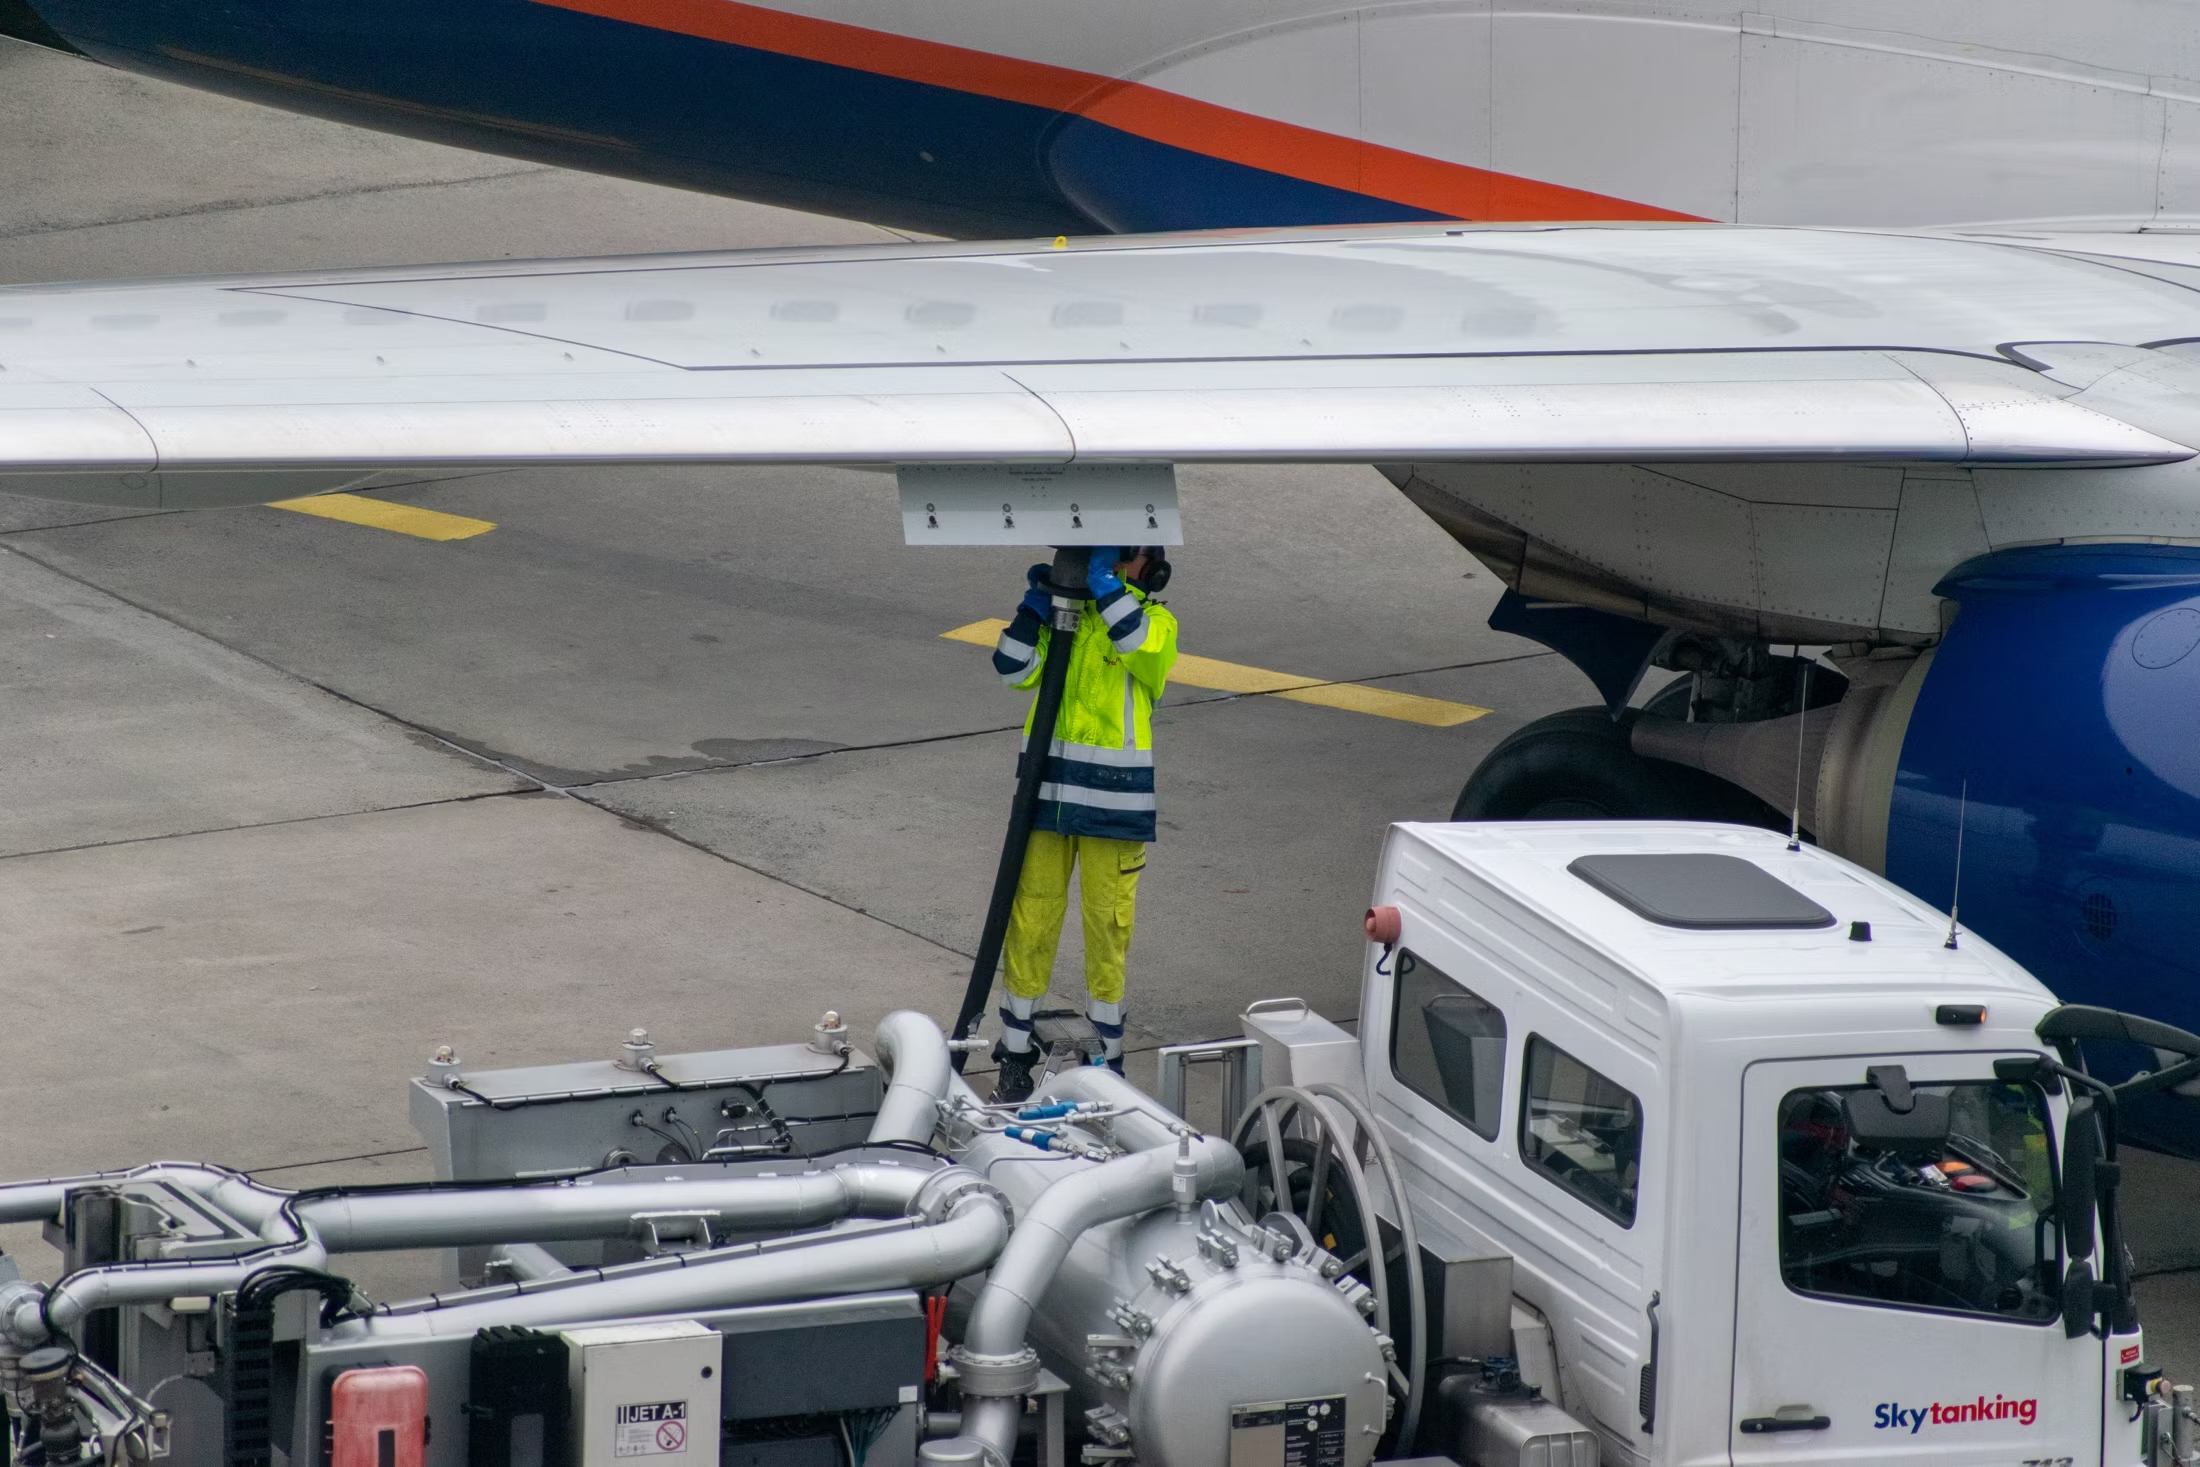
\includegraphics[width=0.5\textwidth]{figures/pressure-refuelling.jpeg}
    \caption{Pressure Refuelling of a Commercial Aircraft. Source: Tom Boon/Simple Flying}\label{fig:pressure-refuelling}
\end{figure}

The aviation industry is undergoing a significant transformation with the
advent of intelligent airports based on highly automated systems. Among these,
automated refuelling systems play a crucial role in ensuring efficient and
accurate refuelling of aircraft. However, one of the main challenges of this
automation process is the accurate detection of the aircraft's refuelling port,
which is relatively small and can easily be obscured by other visual elements
on or near an aircraft. Scanning the entire area of each video frame is both
time-consuming and inaccurate. It is therefore essential to develop a more
efficient and accurate method of locating the refuelling port.

This thesis aims to address this challenge by developing a new AI model that
uses the temporal relationships between successive frames of a video to predict
the location of the refuelling port in subsequent frames. By focusing the
analysis on the most relevant areas of the video sequence, this approach has
the potential to optimise both the speed and accuracy of the refuelling system.

Specific objectives of this thesis include conducting a comprehensive review of
state-of-the-art object detection and tracking methods, designing and
developing a real-time computer vision system capable of accurately detecting
and tracking the pressurised refuelling port of a commercial aircraft, the
implementation and evaluation of deep learning time series models for future
position prediction, the integration of Extended Kalman Filtering (EKF) into
deep learning models to improve the accuracy and robustness of future position
predictions, and the development of a real-time framework for predicting the
future position of the pressurised refuelling port.

By achieving these objectives, this thesis aims to make a significant
contribution to the development of intelligent airport systems and to improve
the efficiency and accuracy of automated refuelling systems at airports, while
reducing computing power requirements. The proposed framework has the potential
to be applied in various scenarios, such as different lighting conditions,
angles and orientations of refuelling ports, making it a versatile and
effective solution to the challenges of automated refuelling systems.

%%%%%%%%%%%%%%%%%%%%%%%%%%%%%%%%%%%%%%%%%%%%%%%%%%%%%%%%%%%%%%%%%%%%%%%%%%%%%%%%
%%%%%%%%%%%%%%%%%%%%%%%%%%%%% LITERATURE REVIEW %%%%%%%%%%%%%%%%%%%%%%%%%%%%%%%%
%%%%%%%%%%%%%%%%%%%%%%%%%%%%%%%%%%%%%%%%%%%%%%%%%%%%%%%%%%%%%%%%%%%%%%%%%%%%%%%%
\chapter{Literature Review}
\section{Automated Refulling Systems in the Aviation Industry}
\subsection{Introduction to Automated Refuelling}

\subsection{Current Technologies and Methods}

\subsection{Challenges in Automated Refuelling}

\subsection{Role of Computer Vision in Automated Refuelling}

\subsection{Future Directions and Innovations}

\newpage
\section{Object Detection and Tracking in Computer Vision}
\subsection{Fundamentals of Object Detection}

\subsection{Techniques and Algorithms for Object Detection}

\subsection{Challenges in Object Detection and Tracking}

\subsection{Applications in the Aviation Industry}

\subsection{Recent Advances and Future Trends}

\newpage
\section{Deep Learning for Time-Series Prediction}
\subsection{Deep Learning Models for Time-Series Prediction}
\subsection{Long Short-Term Memory (LSTM) Networks}
\subsection{Recurrent Neural Networks (RNN)}
\subsection{Transformer Models}
\subsection{Applications in Predictive Modelling}
\subsection{Challenges and Future Research Directions}

%% Back matter
%
% This is where we include references and appendices

\bibliographystyle{CranfieldNumbered.bst}
\bibliography{LaTeX,CUCitations}

\appendix
\chapter{Ethical Approval Letter}
Insert your Ethical Approval Letter as the first appendix.

\chapter{Extra Data}
This is a sample of thesis text. This is a sample of thesis text. This is a
sample of thesis text. This is a sample of thesis text. This is a sample of
thesis text.

This is a sample of thesis text. This is a sample of thesis text. This is a
sample of thesis text. This is a sample of thesis text. This is a sample of
thesis text.

\end{document}

